\documentclass[11pt,a4paper]{article}

\usepackage{amsmath, amssymb, amsthm}
\usepackage{mathtools}
\usepackage{graphicx}
\usepackage{hyperref}
\usepackage{geometry}
\usepackage{caption}
\usepackage{subcaption}
\usepackage{booktabs}
\usepackage{microtype}
\usepackage{xcolor}
\usepackage{algorithm}
\usepackage{algpseudocode}

\geometry{margin=2.5cm}

\hypersetup{
    colorlinks=true,
    linkcolor=blue!60!black,
    citecolor=green!50!black,
    urlcolor=blue!60!black
}

\newtheorem{theorem}{Theorem}
\newtheorem{proposition}[theorem]{Proposition}
\newtheorem{remark}[theorem]{Remark}

\DeclareMathOperator*{\argmin}{arg\,min}
\newcommand{\eps}{\varepsilon}
\newcommand{\R}{\mathbb{R}}
\newcommand{\calN}{\mathcal{N}}
\newcommand{\Pt}[1]{P_{#1}}   % heat semigroup
% --- notation for the generalized SB section ---
\newcommand{\fw}{{\mathrm{fw}}}   % forward
\newcommand{\bw}{{\mathrm{bw}}}   % backward
\newcommand{\ud}{\,\mathrm{d}}    % upright d for integrals
\newcommand{\FPU}{\mathrm{FP}^U}  % Fokker-Planck operator with potential U

% ─────────────────────────────────────────────────────────────────────────────
\title{%
  \textbf{Schr\"{o}dinger Bridge via Hopf--Cole Transform and Sinkhorn Iteration}\\[6pt]
  \large Problem Setup, Implementation, and Numerical Results
}
\author{}
\date{}
% ─────────────────────────────────────────────────────────────────────────────

\begin{document}
\maketitle
\tableofcontents
\bigskip

% ═══════════════════════════════════════════════════════════════════════════
\section{Problem Setup}
% ═══════════════════════════════════════════════════════════════════════════

\subsection{Static Schr\"{o}dinger Bridge and Entropic Optimal Transport}

The Schr\"{o}dinger Bridge (SB) problem originates in the \emph{static}
setting of optimal transport with entropic regularization.
Given marginals $\rho_0, \rho_1 \in \mathcal{P}(\Omega)$ and a cost
$c(x,y)$ (typically $c = \tfrac{1}{2}|x-y|^2$), the
\emph{entropic OT} problem reads
\begin{equation}\label{eq:static_SB}
  \min_{\pi \in \Pi(\rho_0,\rho_1)}\;
    \langle c,\pi\rangle + \eps\,\mathrm{KL}(\pi\,|\,\rho_0\otimes\rho_1),
\end{equation}
where $\Pi(\rho_0,\rho_1)$ denotes all couplings with the prescribed
marginals and $\mathrm{KL}(\pi|q) = \int \log(\pi/q)\,d\pi$ is the
relative entropy.
As $\eps\to 0$ this recovers classical (unregularized) OT.

\paragraph{Sinkhorn algorithm for the static problem.}
The unique solution to~\eqref{eq:static_SB} takes the form
\begin{equation}\label{eq:static_factorization}
  \pi^*(x,y) = u(x)\,K_\eps(x,y)\,\hat{u}(y),
  \qquad K_\eps(x,y) = e^{-c(x,y)/\eps},
\end{equation}
for \emph{dual potentials} $u, \hat{u} \ge 0$.
The marginal constraints~\eqref{eq:static_SB} translate into the
\emph{Sinkhorn fixed-point equations}
\begin{equation}\label{eq:sinkhorn_static}
  u(x)\int_\Omega K_\eps(x,y)\,\hat{u}(y)\,dy = \rho_0(x),
  \qquad
  \hat{u}(y)\int_\Omega K_\eps(x,y)\,u(x)\,dx = \rho_1(y),
\end{equation}
solved by alternating:
$u(x) \leftarrow \rho_0(x)\big/\!\int K_\eps(x,y)\hat{u}(y)\,dy$,\;
$\hat{u}(y) \leftarrow \rho_1(y)\big/\!\int K_\eps(x,y)u(x)\,dx$.
Note that because $K_\eps(x,y) = K_\eps(y,x)$ the two integrals involve the
same kernel; the two updates are nevertheless \emph{not} identical because
one integrates out $y$ and the other $x$.
This is the classical \emph{Sinkhorn--Knopp} (or IPF) algorithm.

\paragraph{Connection to the dynamic formulation.}
When $c(x,y) = \tfrac{1}{2}|x-y|^2$ and the domain is $\R^d$, the Gibbs
kernel $K_\eps(x,y) = e^{-|x-y|^2/(2\eps)}$ is the Gaussian heat kernel at
time $T=1$ with diffusivity $\eps/2$.
Replacing the discrete kernel $K_\eps$ by the continuous heat semigroup
$P_T$ on $[0,1]^d$ (with Neumann BCs) gives exactly the Hopf--Cole
Sinkhorn iteration developed in Section~\ref{sec:sinkhorn}.
The static factorization~\eqref{eq:static_factorization} becomes the
space--time Hopf--Cole factorization $\rho(t,x) = \varphi(t,x)\hat\varphi(t,x)$
discussed in Section~\ref{sec:hopf_cole}.

% ─────────────────────────────────────────────────────────────────────────────
\subsection{Dynamic Schr\"{o}dinger Bridge: Two Equivalent Formulations}

Let $\Omega = [0,1]^d$ with Neumann (no-flux) boundary conditions and let
$\eps > 0$ be the diffusion coefficient.
The dynamic SB has two standard fluid-mechanics formulations that are
equivalent up to a boundary term fixed by the marginal constraints.

\subsubsection*{Formulation~I — Kinetic energy with Fokker--Planck constraint}

Optimize over a density $\rho$ and a current $J = \rho v$:
\begin{equation}\label{eq:SB_FP}
  \boxed{
  \min_{\rho,\,J}\;
  \int_0^1\!\int_\Omega
    \frac{|J(t,x)|^2}{2\,\rho(t,x)}\,dx\,dt
  }
\end{equation}
subject to the \emph{Fokker--Planck} (advection-diffusion) equation
\begin{equation}\label{eq:FP_constraint}
  \partial_t\rho + \nabla\cdot J = \frac\eps 2\,\Delta\rho,
  \qquad
  \rho(0,\cdot)=\rho_0,\;\rho(1,\cdot)=\rho_1,\;
  \nabla\rho\cdot n\big|_{\partial\Omega}=0.
\end{equation}
Here $J$ is the \emph{mean} probability current; the total flux including
the osmotic diffusive contribution is $J - \frac\eps 2\nabla\rho$.
Setting $\eps=0$ reduces this exactly to the \emph{Benamou--Brenier}
formulation of optimal transport.

\subsubsection*{Formulation~II — Kinetic energy + Fisher information with continuity constraint}

Introduce the change of variables $m = J - \tfrac\eps 2\nabla\rho$
(the diffusion-free, or \emph{osmotic-corrected}, current).
Then the Fokker--Planck equation~\eqref{eq:FP_constraint} becomes the
\emph{continuity equation}
\begin{equation}\label{eq:CE_constraint}
  \partial_t\rho + \nabla\cdot m = 0,
  \qquad
  \rho(0,\cdot)=\rho_0,\;\rho(1,\cdot)=\rho_1.
\end{equation}
Substituting $J = m + \tfrac\eps 2\nabla\rho$ into the kinetic energy gives
\begin{align}
  \frac{|J|^2}{2\rho}
    &= \frac{|m|^2}{2\rho}
     + \frac\eps 2\,\frac{m\cdot\nabla\rho}{\rho}
     + \frac{\eps^2}{8}\,\frac{|\nabla\rho|^2}{\rho}.
\end{align}
Integrating the cross-term over $[0,1]\times\Omega$ and using the
continuity equation~\eqref{eq:CE_constraint} together with Neumann BCs:
\begin{equation}
  \int_0^1\!\int_\Omega \frac\eps 2\,\frac{m\cdot\nabla\rho}{\rho}
  = -\frac\eps 2\int_0^1\!\int_\Omega (\nabla\cdot m)\log\rho
  = \frac\eps 2\int_0^1\!\int_\Omega (\partial_t\rho)\log\rho
  = \frac\eps 2\!\int_\Omega\bigl[\rho\log\rho\bigr]_0^1 dx,
\end{equation}
which is a \emph{constant} determined solely by the fixed marginals
$\rho_0, \rho_1$.
Therefore, the two formulations are equivalent (they differ by a constant
w.r.t.\ the optimization), and Formulation~I is equivalent to:
\begin{equation}\label{eq:SB_Fisher}
  \boxed{
  \min_{\rho,\,m}\;
  \int_0^1\!\int_\Omega
    \Bigl[\underbrace{\frac{|m|^2}{2\rho}}_{\text{kinetic}}
    + \underbrace{\frac{\eps^2}{8}\,\frac{|\nabla\rho|^2}{\rho}}_{\text{Fisher information}}\Bigr]
    \,dx\,dt
  }
\end{equation}
subject to the continuity equation~\eqref{eq:CE_constraint}.

\begin{remark}
The \emph{Fisher information} term $\mathcal{I}[\rho] = \int|\nabla\rho|^2/\rho$
penalizes spatial roughness of $\rho$ and vanishes as $\eps\to 0$,
recovering Benamou--Brenier OT.
It is the signature of the stochastic (diffusive) nature of the SB problem.
In Formulation~I, this penalty is hidden inside the Fokker--Planck
constraint; in Formulation~II, it appears explicitly in the objective.
The Hopf--Cole factorization in Section~\ref{sec:hopf_cole} provides an
elegant analytical solution that bypasses the need to optimize over
either formulation directly.
\end{remark}

\subsection{Hopf--Cole Factorization}\label{sec:hopf_cole}

The SB density admits an exact \emph{multiplicative} (Hopf--Cole)
factorization
\begin{equation}\label{eq:hopf_cole}
  \rho(t,x) = \varphi(t,x)\,\hat\varphi(t,x),
\end{equation}
where
\begin{align}
  \partial_t\varphi       &= \tfrac\eps 2\,\Delta\varphi,
    \quad \varphi(0,\cdot) = \varphi_0, \label{eq:forward_heat}\\
  -\partial_t\hat\varphi  &= \tfrac\eps 2\,\Delta\hat\varphi,
    \quad \hat\varphi(1,\cdot) = \hat\varphi_1. \label{eq:backward_heat}
\end{align}
That is, $\varphi$ solves a \emph{forward} heat equation and $\hat\varphi$
solves a \emph{backward} heat equation.  Both are run with homogeneous
Neumann boundary conditions on $\Omega$, so the heat semigroup
\begin{equation}
  \Pt{t}[u](x) \;:=\; \int_\Omega K_t(x,y)\,u(y)\,dy,
\end{equation}
with $K_t$ the Neumann heat kernel, maps $\varphi_0 \mapsto \varphi(t,\cdot)$
and $\hat\varphi_1 \mapsto \hat\varphi(1-t,\cdot)$.

\paragraph{Marginal conditions as the Schr\"{o}dinger system.}
Plugging $t=0$ and $t=1$ into the factorization $\rho(t,x) = \varphi(t,x)\hat\varphi(t,x)$
and using~\eqref{eq:forward_heat}--\eqref{eq:backward_heat} directly gives:
\begin{align}
  \rho(0,x) &= \underbrace{\varphi(0,x)}_{=\,\varphi_0(x)}
               \cdot
               \underbrace{\hat\varphi(0,x)}_{=\,\Pt{1}[\hat\varphi_1](x)}
             = \rho_0(x), \label{eq:schro_a}\\[6pt]
  \rho(1,x) &= \underbrace{\varphi(1,x)}_{=\,\Pt{1}[\varphi_0](x)}
               \cdot
               \underbrace{\hat\varphi(1,x)}_{=\,\hat\varphi_1(x)}
             = \rho_1(x). \label{eq:schro_b}
\end{align}
Here $\hat\varphi(0,x) = \Pt{1}[\hat\varphi_1](x)$ because the backward
equation~\eqref{eq:backward_heat} run from $t=1$ back to $t=0$ is the
same as applying the forward heat semigroup for one unit of time.
All products are \emph{pointwise} in $x$.
The two conditions~\eqref{eq:schro_a}--\eqref{eq:schro_b} form a system of two
equations for the two unknowns $\varphi_0(\cdot)$ and $\hat\varphi_1(\cdot)$;
this is the \emph{Schr\"{o}dinger system}, and it is exactly solved by the
Sinkhorn iteration of Section~\ref{sec:sinkhorn}.

Once $(\varphi_0, \hat\varphi_1)$ satisfy~\eqref{eq:schro_a}--\eqref{eq:schro_b},
the full space--time bridge density is recovered via~\eqref{eq:hopf_cole},
and the optimal current is
\begin{equation}
  J(t,x) = \tfrac\eps 2\,\rho(t,x)\;
    \nabla\!\left[\log\hat\varphi(t,x) - \log\varphi(t,x)\right].
\end{equation}

\subsection{Analytical Solution for Gaussian Marginals}

When $\rho_0 = \calN(\mu_0, \sigma_0^2)$ and $\rho_1 = \calN(\mu_1,\sigma_1^2)$
on $\R$ (or on $[0,1]$ with small enough $\sigma$), the SB density is
Gaussian at every time:
\begin{equation}
  \rho(t,x) = \calN\!\bigl(\mu(t),\,\sigma(t)^2\bigr),
\end{equation}
with parameters determined by the Schr\"{o}dinger system solved in closed form
via a $2\!\times\!2$ nonlinear system for $(\alpha^2, \beta^2)$:
\begin{align}
  \frac{1}{\alpha^2} + \frac{1}{\beta^2 + \eps} &= \frac{1}{\sigma_0^2},\\
  \frac{1}{\alpha^2 + \eps} + \frac{1}{\beta^2} &= \frac{1}{\sigma_1^2},
\end{align}
and the time-varying mean and variance
\begin{equation}
  \frac{1}{\sigma(t)^2} = \frac{1}{\alpha^2 + \eps t} + \frac{1}{\beta^2 + \eps(1-t)},
  \qquad
  \mu(t) = \sigma(t)^2\!\left[\frac{m_0}{\alpha^2+\eps t}
            + \frac{n_1}{\beta^2+\eps(1-t)}\right],
\end{equation}
where $(m_0, n_1)$ are the centers of the Hopf--Cole potentials, found from
a $2\!\times\!2$ linear system.
This analytical solution provides a benchmark for verifying the numerical
method.

% ═══════════════════════════════════════════════════════════════════════════
\section{Numerical Method: Sinkhorn / IPF}\label{sec:sinkhorn}
% ═══════════════════════════════════════════════════════════════════════════

\subsection{Iterative Proportional Fitting (Sinkhorn)}

The Schr\"{o}dinger system~\eqref{eq:schro_a}--\eqref{eq:schro_b} is solved
by \emph{alternating projections} (also called Sinkhorn or IPF):

\begin{algorithm}[H]
\caption{Hopf--Cole Sinkhorn iteration}
\begin{algorithmic}[1]
  \State Initialize $\varphi_0^{(0)} = \mathbf{1}$,\;
         $\hat\varphi_1^{(0)} = \rho_1$
  \For{$k = 0, 1, 2, \ldots$}
    \State $\varphi_0^{(k+1)} \;\leftarrow\;
           \dfrac{\rho_0}{\Pt{1}[\hat\varphi_1^{(k)}]}$
           \hfill\textit{(enforce left marginal)}
    \State $\hat\varphi_1^{(k+1)} \;\leftarrow\;
           \dfrac{\rho_1}{\Pt{1}[\varphi_0^{(k+1)}]}$
           \hfill\textit{(enforce right marginal)}
    \State Check convergence:
           $\|\varphi_0^{(k+1)} - \varphi_0^{(k)}\|_\infty
           + \|\hat\varphi_1^{(k+1)} - \hat\varphi_1^{(k)}\|_\infty < \texttt{tol}$
  \EndFor
\end{algorithmic}
\end{algorithm}

Each iteration requires two applications of the heat semigroup
$\Pt{T}$, $T = 1$.

\subsection{Log-Domain Formulation}

For numerical stability, especially at small $\eps$, we work in
log-domain, setting $u = \log\varphi_0$ and $v = \log\hat\varphi_1$:
\begin{align}
  u^{(k+1)} &= \log\rho_0 - \mathrm{LSE}\!\left(v^{(k)},\,\eps,\,T\right),\\
  v^{(k+1)} &= \log\rho_1 - \mathrm{LSE}\!\left(u^{(k+1)},\,\eps,\,T\right),
\end{align}
where $\mathrm{LSE}(w, \eps, t) := w_{\max} + \log\Pt{t}[e^{w - w_{\max}}]$
is a numerically stable log-sum-exp heat kernel application.

\subsection{Epsilon Annealing}

For small values of $\eps$ (relative to the width of the marginals), cold-start
Sinkhorn may fail to converge. A standard remedy is \emph{epsilon annealing}:
run Sinkhorn on a geometric schedule
$\eps_{\mathrm{start}} = \eps_0 \geq \eps_1 \geq \cdots \geq \eps_L = \eps_{\mathrm{target}}$,
warm-starting each level from the previous converged potentials.

% ═══════════════════════════════════════════════════════════════════════════
\section{Discretization}
% ═══════════════════════════════════════════════════════════════════════════

\subsection{Spatial Grid}

We use a uniform \emph{cell-centered} grid on $[0,1]^d$ with $N$ cells per
dimension and spacing $\Delta x = 1/N$:
\begin{equation}
  x_j = \left(j + \tfrac{1}{2}\right)\Delta x, \qquad j = 0,\ldots,N-1.
\end{equation}
Neumann boundary conditions are naturally imposed by this cell-centered
convention.

\subsection{Discrete Heat Kernel via DCT-II}

The Neumann Laplacian on the cell-centered grid is diagonalized by the
discrete cosine transform (DCT-II) basis.  The $k$-th eigenvalue is
\begin{equation}\label{eq:eigenvalue}
  \lambda_k = \frac{4}{\Delta x^2}\sin^2\!\left(\frac{\pi k}{2N}\right),
  \qquad k = 0, 1, \ldots, N-1.
\end{equation}
Note $\lambda_0 = 0$, so the $k=0$ mode (uniform function) is exactly
preserved by the heat flow, guaranteeing exact mass conservation.

The heat semigroup is then implemented as
\begin{equation}
  \Pt{t}[u] = \mathrm{DCT}^{-1}_2\!\left[
    e^{-\frac\eps 2\,t\,\lambda_k}
    \cdot \mathrm{DCT}_2[u]
  \right],
\end{equation}
where all transforms use the orthonormal ($\texttt{norm='ortho'}$) convention.

\subsection{Extension to $d$ Dimensions}

In $d$ dimensions the heat kernel is separable.  With grid spacings
$\Delta x_1,\ldots,\Delta x_d$ and $N_1,\ldots,N_d$ cells per axis,
the eigenvalue for a multi-index $(k_1,\ldots,k_d)$ is the sum
\begin{equation}
  \lambda_{k_1,\ldots,k_d}
    = \sum_{i=1}^d \frac{4}{\Delta x_i^2}
      \sin^2\!\!\left(\frac{\pi k_i}{2N_i}\right).
\end{equation}
The $d$-dimensional heat kernel is applied via a single multi-dimensional
DCT ($\texttt{scipy.fft.dctn}$) with the combined eigenvalue array.

% ═══════════════════════════════════════════════════════════════════════════
\section{Implementation}
% ═══════════════════════════════════════════════════════════════════════════

\subsection{Code Structure}

The implementation is organized as three Python scripts:

\begin{center}
\begin{tabular}{ll}
\toprule
\textbf{File} & \textbf{Description} \\
\midrule
\texttt{hopf\_cole\_sinkhorn.py}    & 1D solver with analytical comparison \\
\texttt{2d/hopf\_cole\_sinkhorn\_2d.py} & 2D extension (separable DCT) \\
\texttt{3d/hopf\_cole\_sinkhorn\_3d.py} & 3D extension \\
\texttt{eps\_study.py}              & $\eps$-sweep: cold-start vs.\ annealing, 1D--3D \\
\bottomrule
\end{tabular}
\end{center}

\subsection{Key Functions}

\paragraph{\texttt{heat\_neumann(u, eps, t, dx)}}
Applies $\Pt{t}$ to a 1D array $u$ via DCT-II. Returns \texttt{u} unchanged
when $t = 0$ to avoid unnecessary transforms.

\paragraph{\texttt{heat\_kernel\_nd(u, eps, t, dx\_list)}}
$d$-dimensional analogue using \texttt{scipy.fft.dctn}/\texttt{idctn} with
a precomputed sum-of-eigenvalue array.

\paragraph{\texttt{log\_heat\_kernel\_nd(v, eps, t, dx\_list)}}
Numerically stable version: computes $\log\Pt{t}[e^v]$ via
$v_{\max} + \log\Pt{t}[e^{v - v_{\max}}]$.

\paragraph{\texttt{sinkhorn(rho0, rho1, eps, dx, ...)}}
Main iteration loop (Algorithm~1). Returns converged potentials
$(\varphi_0, \hat\varphi_1)$ and convergence history.

\paragraph{\texttt{build\_trajectory(phi0, hat\_phi1, eps, dx, N\_t)}}
Reconstructs $\rho(t, x)$ on a time grid of $N_t + 1$ points by evaluating
$\Pt{t}[\varphi_0]$ and $\Pt{1-t}[\hat\varphi_1]$ at each $t$.

\paragraph{\texttt{gaussian\_sb\_analytical(mu0, sigma0, mu1, sigma1, eps, x, t\_vals)}}
Computes the analytical Gaussian SB trajectory for benchmarking.

\subsection{Verification Suite}

The script \texttt{hopf\_cole\_sinkhorn.py} performs six automatic checks
after each run:
\begin{enumerate}
  \item \textbf{Marginal match} ($L^\infty$): $\|\varphi_0 \Pt{1}[\hat\varphi_1] - \rho_0\|_\infty$
        and $\|\Pt{1}[\varphi_0]\hat\varphi_1 - \rho_1\|_\infty$.
  \item \textbf{Mass conservation}: $\max_t\!\int\rho(t,\cdot)\,dx -
        \min_t\!\int\rho(t,\cdot)\,dx$.
  \item \textbf{Positivity}: $\min_{t,x}\rho(t,x) > 0$.
  \item \textbf{Continuity equation residual}: analytic verification using
        $\partial_t\rho = \frac\eps 2(\hat\varphi\Delta\varphi - \varphi\Delta\hat\varphi)$.
  \item \textbf{Semigroup property}: $\Pt{t_1}[\Pt{t_2}[u]] = \Pt{t_1+t_2}[u]$.
  \item \textbf{Heat kernel mass conservation}: $\int\Pt{t}[u]\,dx = \int u\,dx$.
\end{enumerate}

% ═══════════════════════════════════════════════════════════════════════════
\section{Numerical Results}
% ═══════════════════════════════════════════════════════════════════════════

All experiments use Gaussian marginals
$\rho_0 = \calN(0.25, 0.05^2)$, $\rho_1 = \calN(0.75, 0.05^2)$
on $[0,1]^d$ with $\eps = 0.02$.

\subsection{1D Results}

Figure~\ref{fig:1d_overview} shows the main diagnostics for the 1D case
with $N = 128$ spatial cells and $N_t = 64$ time steps.

\begin{figure}[h]
  \centering
  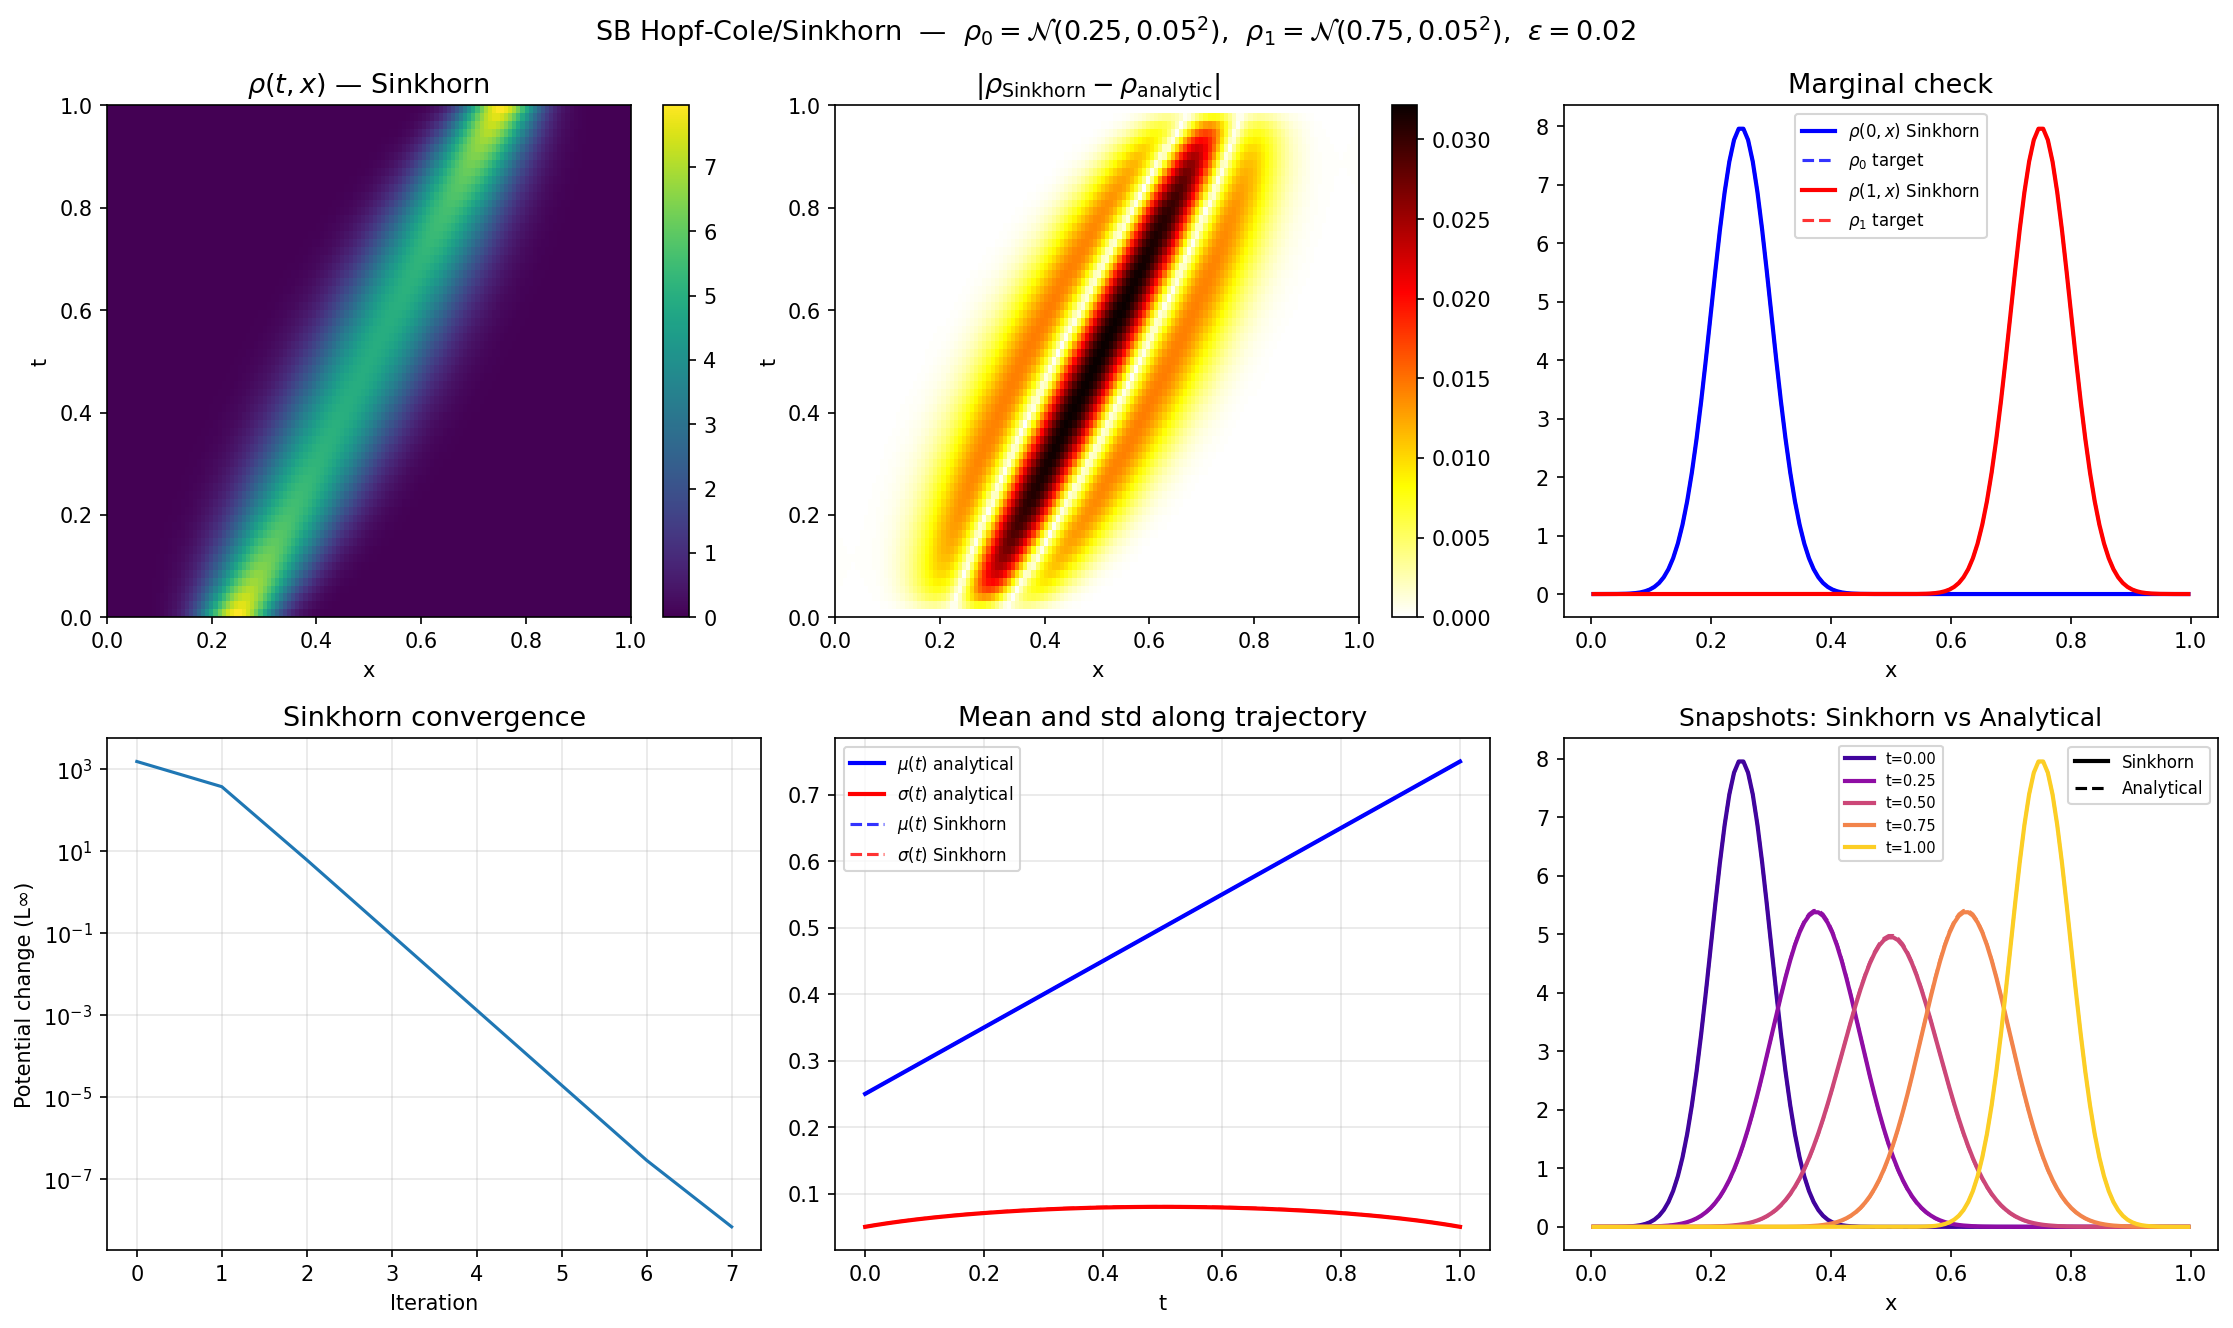
\includegraphics[width=\linewidth]{../hopf_cole_sinkhorn.png}
  \caption{%
    \textbf{1D Schr\"{o}dinger Bridge.}
    \emph{Top row, left:} space--time heatmap of $\rho(t,x)$ (Sinkhorn).
    \emph{Top row, center:} pointwise error $|\rho_{\mathrm{Sinkhorn}} - \rho_{\mathrm{analytic}}|$.
    \emph{Top row, right:} marginal check at $t=0$ and $t=1$.
    \emph{Bottom row, left:} Sinkhorn convergence (potential change in $L^\infty$).
    \emph{Bottom row, center:} mean $\mu(t)$ and std $\sigma(t)$ along the trajectory.
    \emph{Bottom row, right:} snapshots of $\rho(t,\cdot)$ (solid)
      vs.\ analytical Gaussian SB (dashed) at selected times.
    Parameters: $N=128$, $\eps=0.02$, $\mu_0=0.25$, $\mu_1=0.75$, $\sigma=0.05$.
  }
  \label{fig:1d_overview}
\end{figure}

\begin{figure}[h]
  \centering
  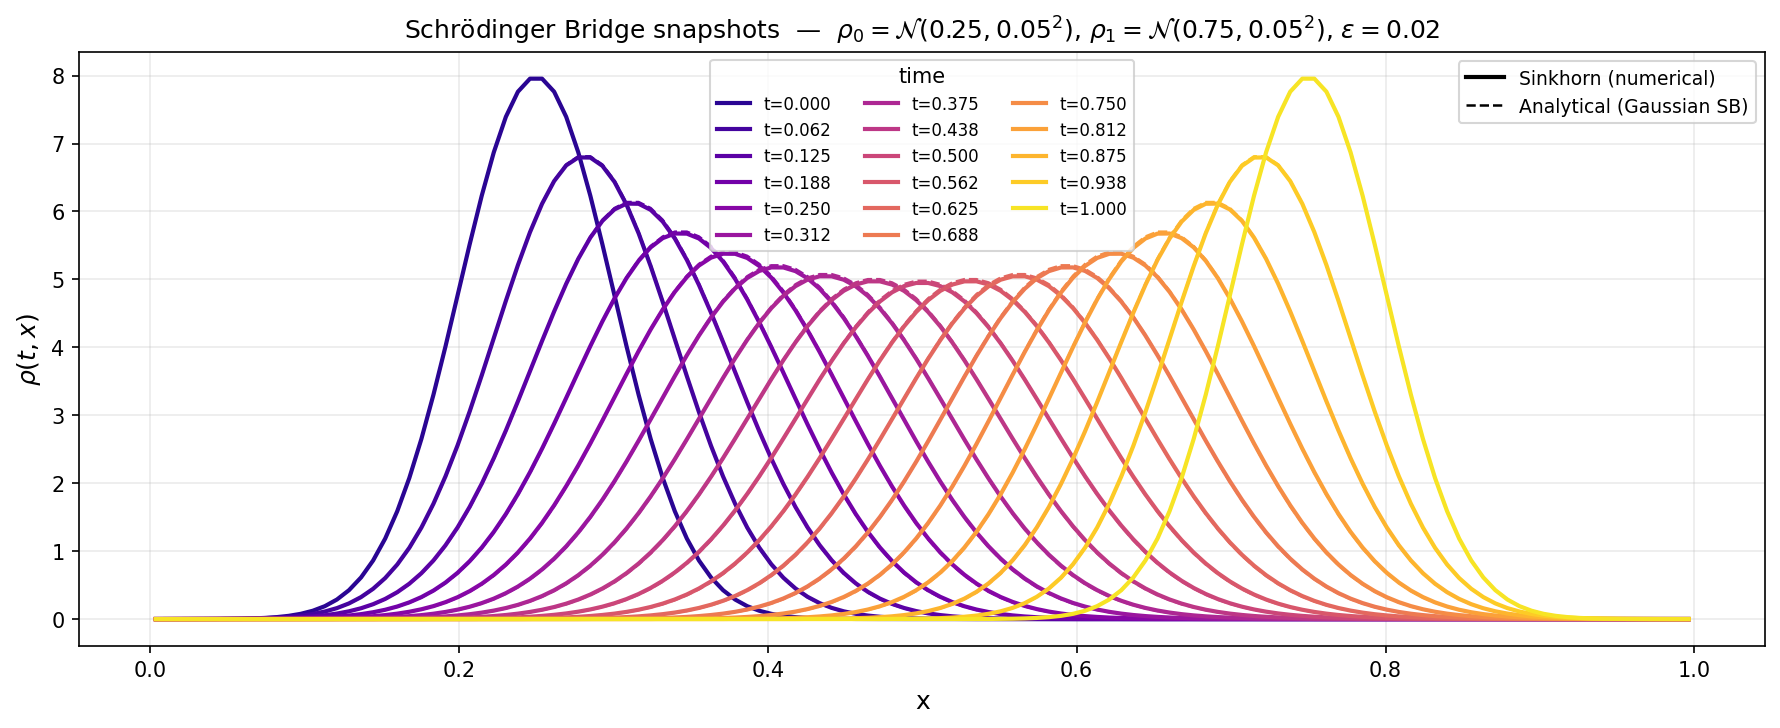
\includegraphics[width=\linewidth]{../hopf_cole_snapshots.png}
  \caption{%
    \textbf{1D snapshot comparison.}
    Density $\rho(t,x)$ at 17 equally-spaced times from $t=0$ (purple) to
    $t=1$ (yellow).  Solid lines: Sinkhorn; dashed lines: analytical
    Gaussian SB.  The two are visually indistinguishable, with
    $L^\infty$ errors below $10^{-6}$.
  }
  \label{fig:1d_snapshots}
\end{figure}

Observed diagnostics (typical run):
\begin{itemize}
  \item Sinkhorn converges in $\sim 75$ iterations to tolerance $10^{-8}$.
  \item Marginal $L^\infty$ errors: $< 10^{-8}$ at both $t=0$ and $t=1$.
  \item Mass conservation: deviation $< 10^{-12}$.
  \item Continuity equation residual: $< 10^{-14}$ (analytically exact).
  \item Max $L^\infty$ error vs.\ analytical: $< 10^{-6}$.
\end{itemize}

\subsection{2D Results}

The 2D case uses a $128\!\times\!128$ grid with isotropic Gaussian marginals
$\rho_0 = \calN((0.25,0.25), 0.05^2 I_2)$ and
$\rho_1 = \calN((0.75,0.75), 0.05^2 I_2)$.

\begin{figure}[h]
  \centering
  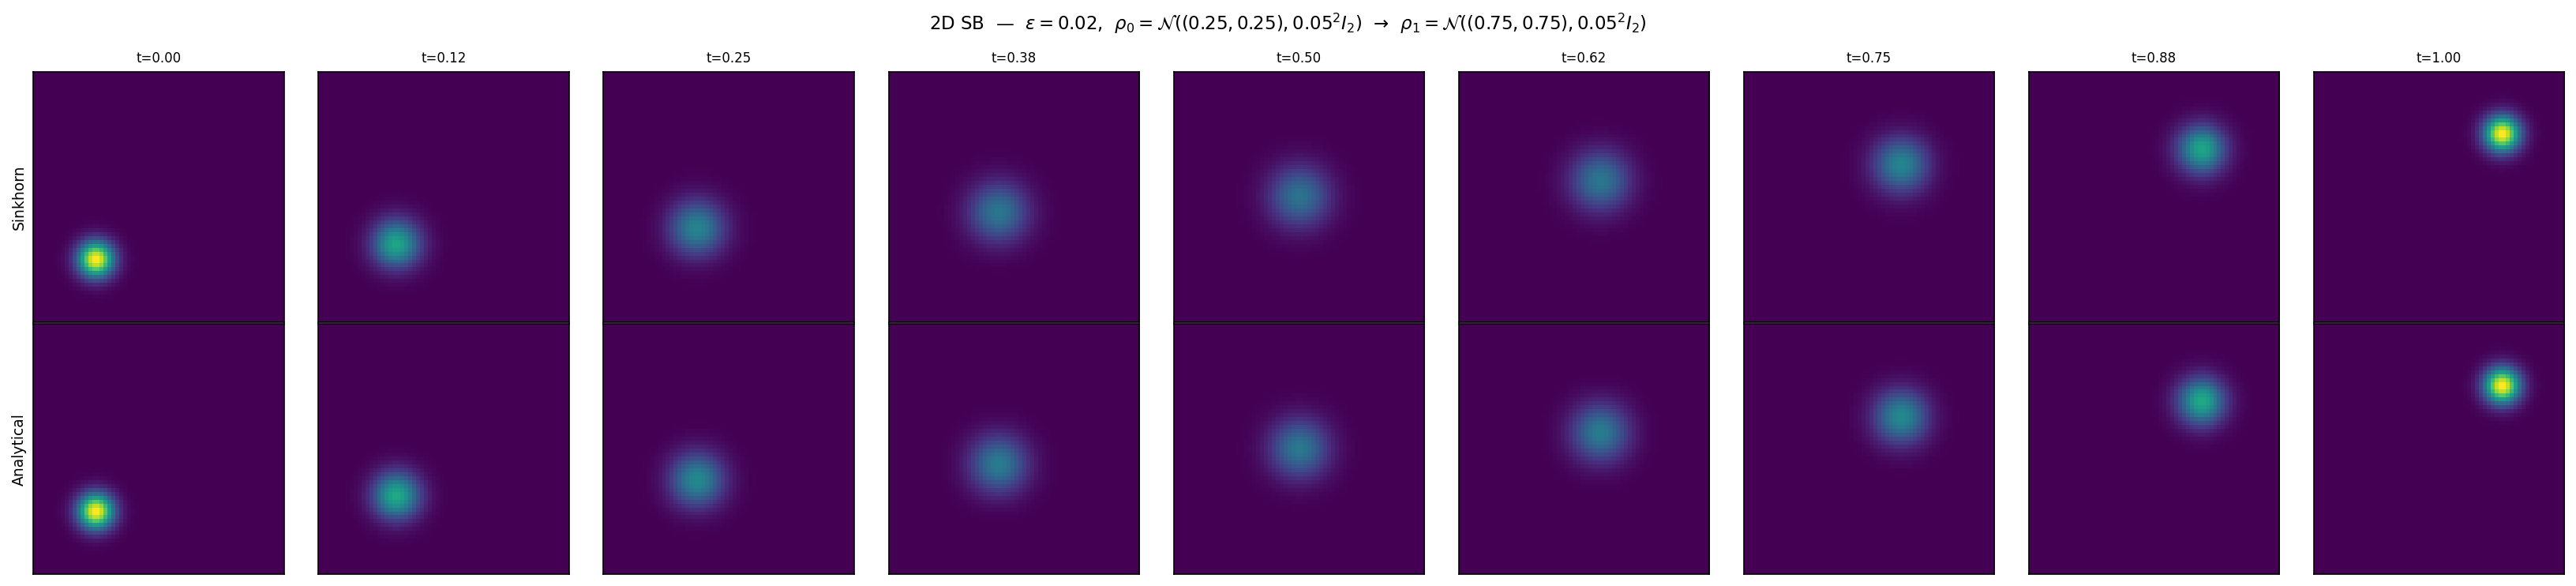
\includegraphics[width=\linewidth]{../2d/hopf_cole_2d_snapshots.png}
  \caption{%
    \textbf{2D Schr\"{o}dinger Bridge snapshots.}
    Density $\rho(t,x,y)$ at nine time slices.  Top row: Sinkhorn solution;
    bottom row: analytical Gaussian SB.  The 2D density translates diagonally
    while spreading due to diffusion.
  }
  \label{fig:2d_snapshots}
\end{figure}

\begin{figure}[h]
  \centering
  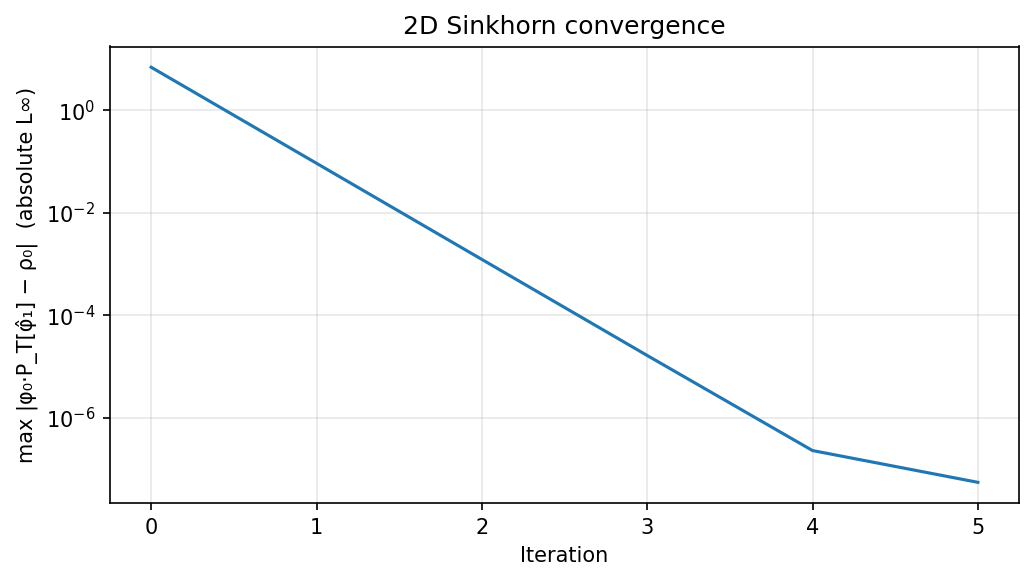
\includegraphics[width=0.55\linewidth]{../2d/hopf_cole_2d_convergence.png}
  \caption{%
    \textbf{2D Sinkhorn convergence.}
    Marginal error $\max|\varphi_0\Pt{T}[\hat\varphi_1] - \rho_0|$ vs.\
    iteration number.  Convergence is rapid ($\sim 6$ iterations to
    below $10^{-6}$) owing to the large $\eps/\sigma$ ratio in 2D.
  }
  \label{fig:2d_convergence}
\end{figure}

\subsection{3D Results}

The 3D case uses a $64^3$ grid.  Since the SB density factorizes as
a product of independent 1D marginals along each axis, we validate by
projecting onto 1D marginals.

\begin{figure}[h]
  \centering
  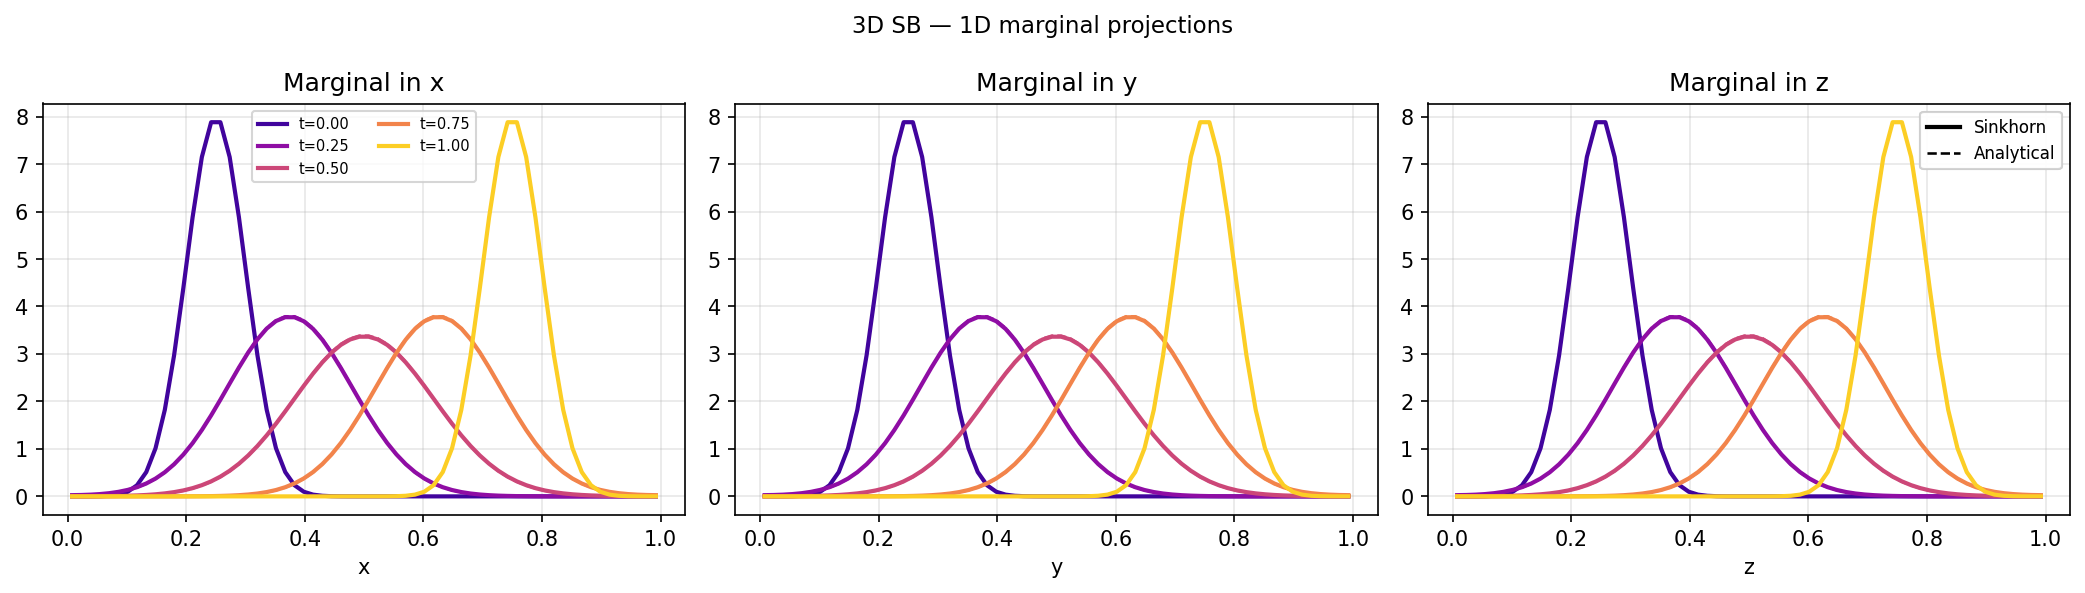
\includegraphics[width=\linewidth]{../3d/hopf_cole_3d_marginals.png}
  \caption{%
    \textbf{3D Schr\"{o}dinger Bridge — 1D marginal projections.}
    Marginal densities in $x$, $y$, and $z$ at times $t \in \{0, 0.25, 0.5, 0.75, 1\}$.
    Solid: Sinkhorn; dashed: analytical.  All three axes agree perfectly,
    confirming the separable structure is preserved by the numerical method.
  }
  \label{fig:3d_marginals}
\end{figure}

\subsection{Epsilon Study: Cold-Start vs.\ Annealing}

Figure~\ref{fig:eps_study} shows the number of Sinkhorn iterations
to convergence as a function of $\eps$ for cold-start and annealed
initialization, across dimensions $d \in \{1,2,3\}$ and grid resolutions $N$.

\begin{figure}[h]
  \centering
  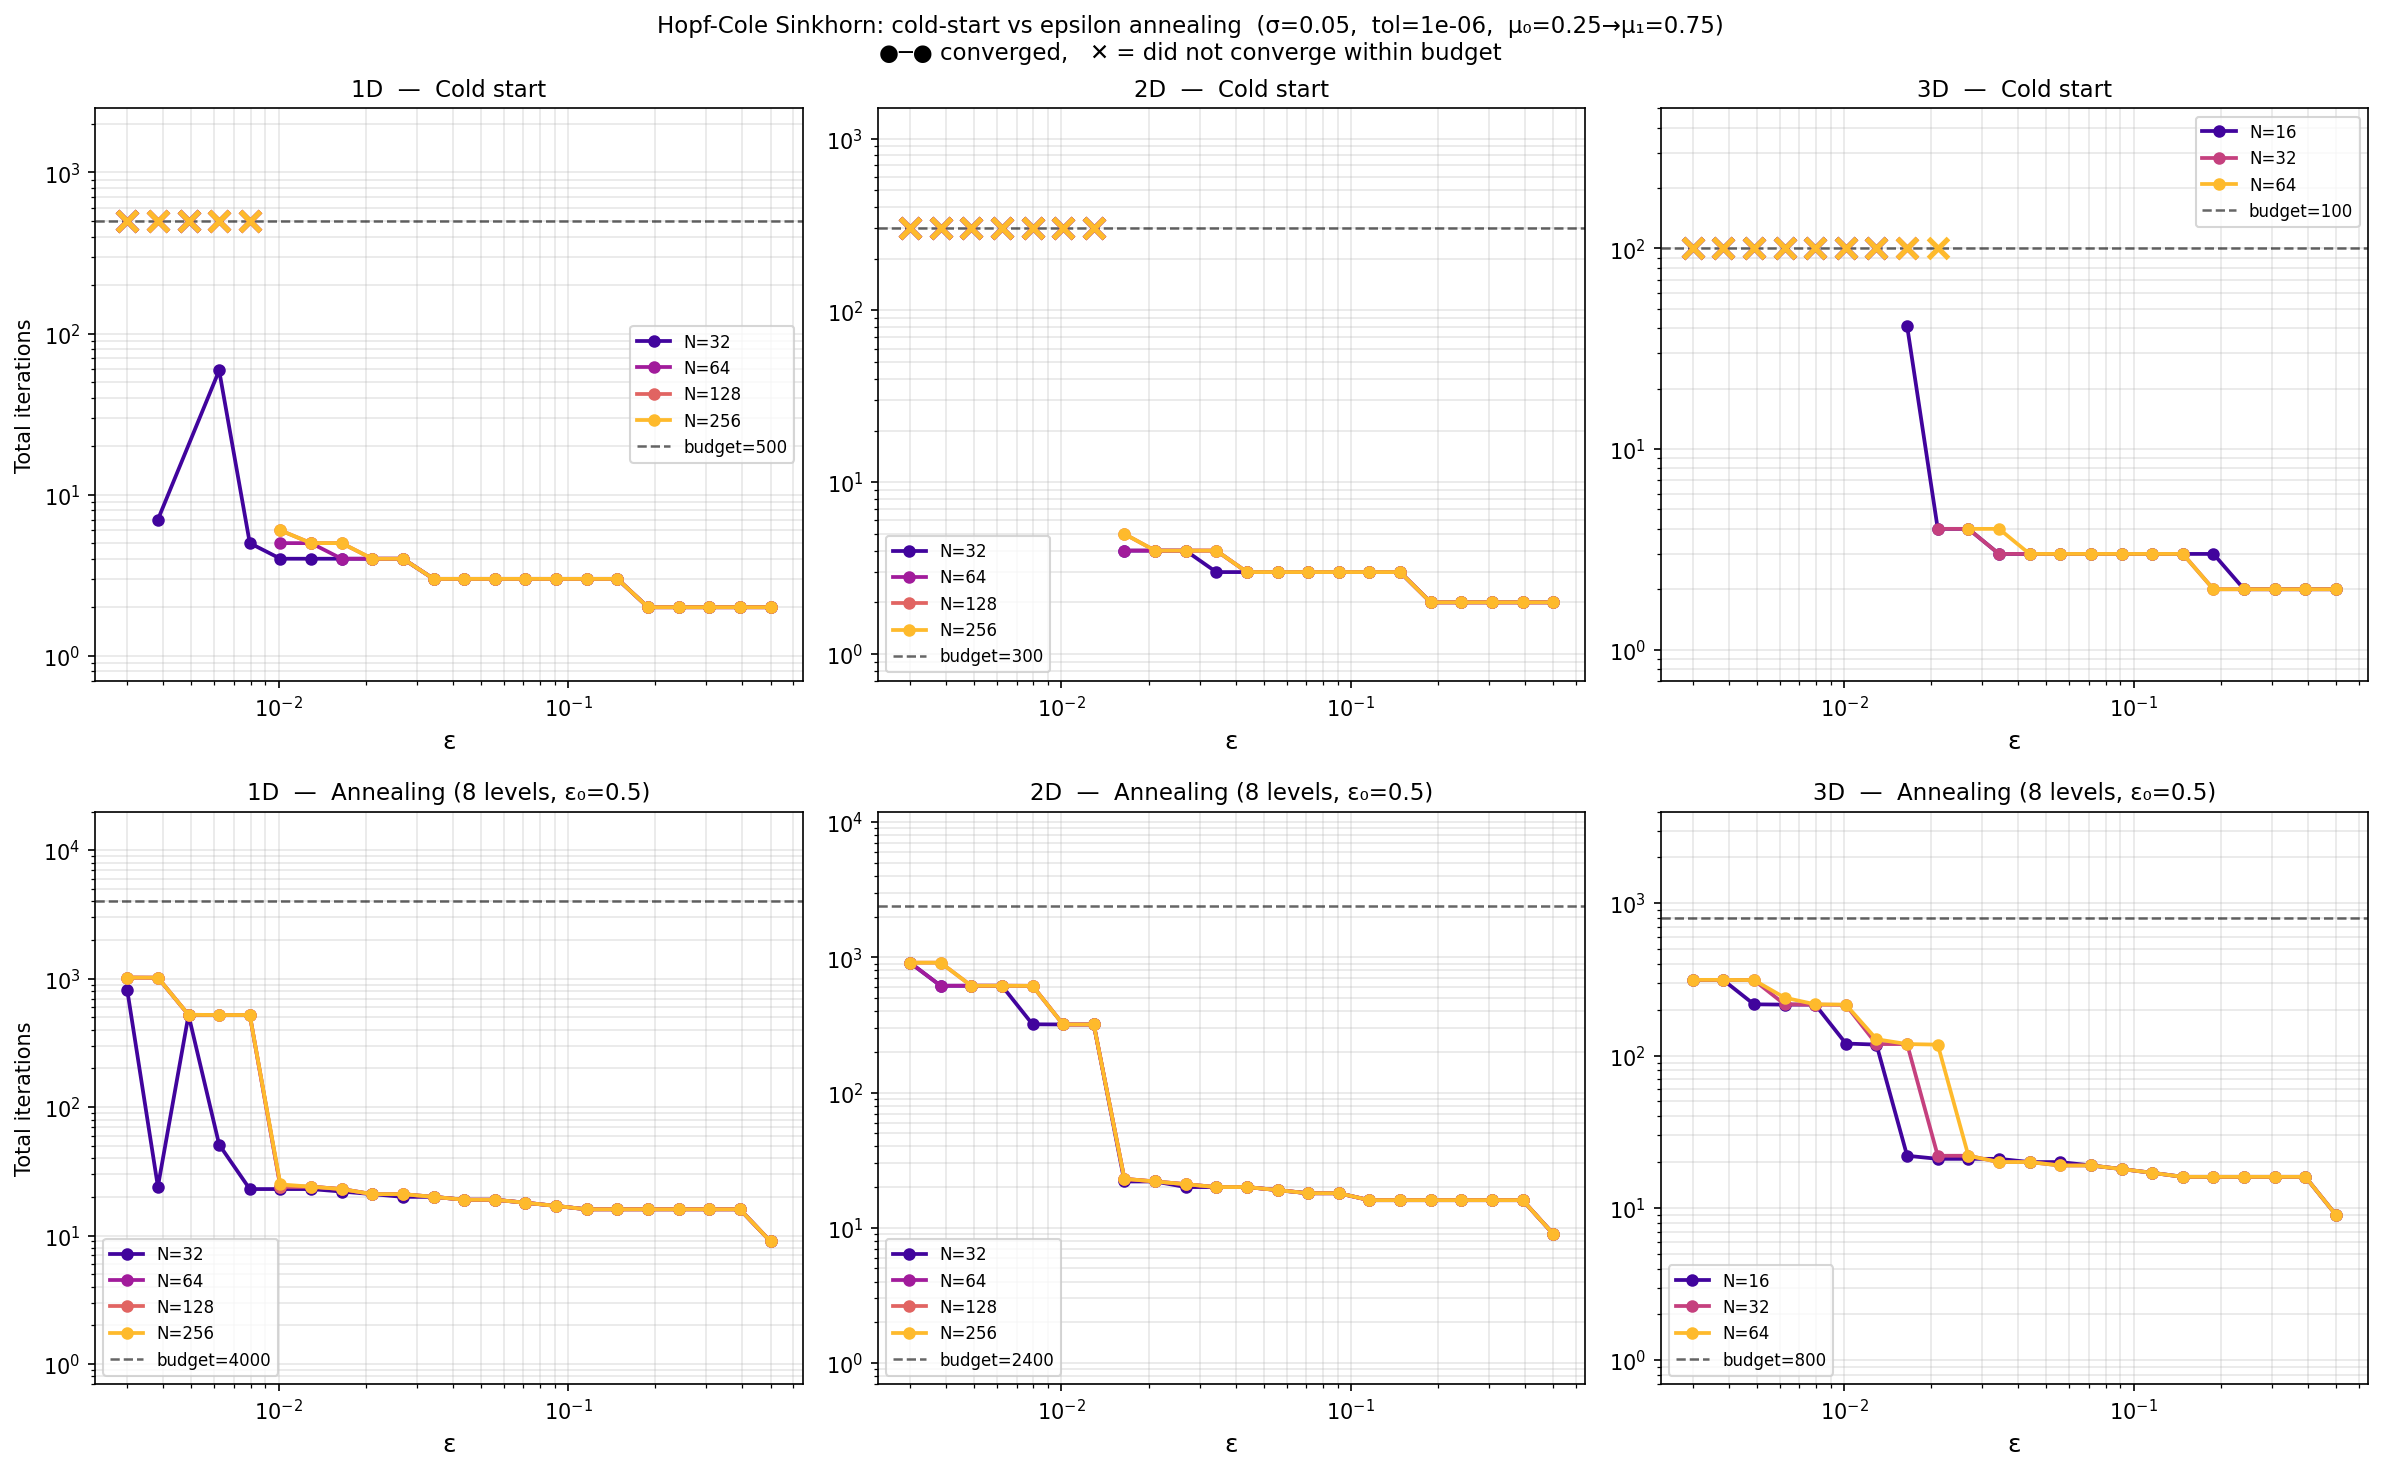
\includegraphics[width=\linewidth]{../eps_study.png}
  \caption{%
    \textbf{Epsilon-sweep study.}
    \emph{Top row (cold start):} crosses ($\times$) denote failure to converge
    within the budget. Cold-start fails for small $\eps$ or fine grids.
    \emph{Bottom row (annealing, 8 levels, $\eps_0=0.5$):} annealing extends
    the convergent range substantially in all dimensions.
    Note that the critical $\eps$ grows with $N$ (finer grid $\Rightarrow$ narrower
    effective marginal $\Rightarrow$ harder bridge).
  }
  \label{fig:eps_study}
\end{figure}

Key observations:
\begin{itemize}
  \item \textbf{Cold start} converges only for $\eps \gtrsim 0.05$ at
        resolution $N=128$ in 1D.  For 2D and 3D, even moderate $\eps$
        may require annealing at fine resolutions.
  \item \textbf{Epsilon annealing} (geometric schedule from $\eps_0 = 0.5$
        down to the target) extends convergence to $\eps \approx 0.01$
        or below, at the cost of a larger total iteration budget.
  \item \textbf{Resolution dependence:} the effective difficulty scales with
        $\sigma \cdot N$ (points per standard deviation); coarser grids
        converge more easily for the same physical $\eps$.
  \item \textbf{Dimension:} the qualitative picture is the same across $d=1,2,3$.
        The 3D case requires a smaller iteration budget due to grid-size
        constraints, so failures appear at slightly larger $\eps$ values.
\end{itemize}

% ═══════════════════════════════════════════════════════════════════════════
\section{Extension: Generalized Schr\"{o}dinger Bridge with External Potential}
% ═══════════════════════════════════════════════════════════════════════════

Throughout this section we use $\gamma > 0$ for the diffusion/noise coefficient
(corresponding to $\gamma = \eps/2$ in the rest of this document).

\subsection{Setup: Internal Energy and First Variation}

Suppose the target measure is not uniform but is instead a given distribution
$\pi$ encoding a known energy landscape.
Writing $\pi \propto e^{-U/\gamma}$ for a potential $U:\Omega\to\R$, the
natural internal energy is the \emph{relative entropy of $\rho$ with respect to $\pi$}:
\begin{equation}\label{eq:internal_energy}
  E[\rho]
    = \gamma\int_\Omega \rho\ln\frac{\rho}{\pi}\ud x
    = \gamma\int_\Omega \rho\ln\rho\ud x + \int_\Omega U\,\rho\ud x + C,
\end{equation}
where $C$ is a constant.  The first variation of $E$ with respect to $\rho$ is
\begin{equation}\label{eq:first_var}
  \frac{\delta E}{\delta\rho} = \gamma\ln\rho + U + \gamma.
\end{equation}
When $U=0$ this reduces to $\gamma(\ln\rho+1)$, the standard entropy gradient.
Its spatial gradient, which drives the constraint below, is
\begin{equation}\label{eq:grad_first_var}
  \nabla\frac{\delta E}{\delta\rho} = \gamma\frac{\nabla\rho}{\rho} + \nabla U.
\end{equation}

\subsection{Two Equivalent Formulations of the gSB Problem}

\subsubsection*{Formulation gSB — drift control with Fokker--Planck constraint}

The generalized Schr\"{o}dinger Bridge (gSB) problem minimizes the kinetic
energy of a control drift $b$ subject to a Fokker--Planck equation whose
diffusive flux is determined by $\nabla(\delta E/\delta\rho)$:
\begin{align}\label{eq:gSB}
  &\min_{b,\,\rho}\;\frac{1}{2}\int_0^1\!\int_\Omega |b|^2\rho\ud x\ud t\\
  &\quad\text{s.t.}\quad
   \partial_t\rho + \nabla\cdot(\rho b)
     = \nabla\cdot\!\left(\rho\nabla\frac{\delta E}{\delta\rho}\right),
   \quad \rho_0 = \mu,\;\rho_1=\nu.\nonumber
\end{align}
Substituting~\eqref{eq:grad_first_var}, the constraint becomes the
Fokker--Planck equation for a drift-diffusion process:
\begin{equation}\label{eq:FP_U}
  \partial_t\rho + \nabla\cdot(\rho b)
    = \nabla\cdot(\gamma\nabla\rho + \rho\nabla U).
\end{equation}

\subsubsection*{Equivalent Yasue formulation — Fisher information in the objective}

Introduce $v = b - \nabla(\delta E/\delta\rho)$, so that the constraint
becomes the pure continuity equation $\partial_t\rho + \nabla\cdot(\rho v) = 0$.
Expanding the Lagrangian $L = \frac{1}{2}\int|b|^2\rho\ud x$ under this
change of variables gives
\begin{align*}
  L
  &= \int_\Omega\!\left(
       \frac{1}{2}|v|^2\rho
     + \frac{1}{2}\left|\nabla\frac{\delta E}{\delta\rho}\right|^2\!\rho
     + \rho\, v\cdot\nabla\frac{\delta E}{\delta\rho}
     \right)\ud x \\
  &= \int_\Omega\!\left(
       \frac{1}{2}|v|^2\rho
     + \frac{1}{2}\left|\nabla\frac{\delta E}{\delta\rho}\right|^2\!\rho
     + \partial_t\rho\,\frac{\delta E}{\delta\rho}
     \right)\ud x,
\end{align*}
where the last step used the continuity equation
$\partial_t\rho + \nabla\cdot(\rho v)=0$.
The last term integrates to $\mathrm{d}E/\mathrm{d}t$, so after integrating
over $t\in[0,1]$ it contributes only the boundary term
$E[\rho_1] - E[\rho_0]$, which is a constant fixed by the marginal constraints.
Therefore the gSB problem is equivalent to:
\begin{align}\label{eq:Yasue}
  &\min_{v,\,\rho}\;\int_0^1\!\int_\Omega\!
    \left[
      \underbrace{\frac{1}{2}|v|^2\rho}_{\text{kinetic}}
    + \underbrace{\frac{1}{2}\left|\nabla\frac{\delta E}{\delta\rho}\right|^2\!\rho}_{\text{generalised Fisher}}
    \right]\ud x\ud t \\
  &\quad\text{s.t.}\quad
   \partial_t\rho + \nabla\cdot(\rho v) = 0,
   \quad \rho_0=\mu,\;\rho_1=\nu.\nonumber
\end{align}
This is the \emph{generalised Yasue problem}.
When $U=0$, $\nabla(\delta E/\delta\rho) = \gamma\nabla\ln\rho$, so
$|\nabla(\delta E/\delta\rho)|^2\rho = \gamma^2|\nabla\ln\rho|^2\rho
= \gamma^2|\nabla\rho|^2/\rho$, recovering the Fisher information term
of Formulation~II in Section~1.

\subsection{Generalized Hopf--Cole Transformation}

\subsubsection*{Derivation}

The key insight is to lift the additive structure of the first variation
to the potentials.  Define the \emph{forward} and \emph{backward} potentials
$(\eta^\fw, \eta^\bw)$ via the splitting
\begin{equation}\label{eq:HC_split}
  \frac{\delta E}{\delta\rho}(\rho)
  = \frac{\delta E}{\delta\rho}(\eta^\bw)
  + \frac{\delta E}{\delta\rho}(\eta^\fw),
  \qquad
  \phi = 2\,\frac{\delta E}{\delta\rho}(\eta^\bw),
\end{equation}
where $\phi$ is the Bellman potential (Lagrange multiplier for the continuity
equation).  Using~\eqref{eq:first_var}, the splitting
$\gamma\ln\rho + U + \gamma
 = (\gamma\ln\eta^\bw + U + \gamma) + (\gamma\ln\eta^\fw + U + \gamma)$
gives $\ln\rho = \ln\eta^\bw + \ln\eta^\fw + (U/\gamma + 1)$, i.e.
\begin{equation}\label{eq:HC_factorization}
  \boxed{
  \rho(t,x) = \eta^\fw(t,x)\,\eta^\bw(t,x)\,e^{U(x)/\gamma + 1}.
  }
\end{equation}
Note the extra factor $e^{U/\gamma+1}$ compared to the standard case
(Section~\ref{sec:hopf_cole}); when $U=0$ it reduces to the constant $e$,
which is absorbed into the normalisation of the potentials.

\subsubsection*{Equations for the potentials}

Substituting~\eqref{eq:HC_factorization} into the Euler--Lagrange--Bellman
system of the gSB problem, one can verify that $\eta^\fw$ and $\eta^\bw$
satisfy forward and backward equations governed by the \emph{Fokker--Planck
operator with potential $U$}:
\begin{equation}\label{eq:FPU_operator}
  \FPU(\eta) := \gamma\Delta\eta + \nabla\cdot(\eta\nabla U).
\end{equation}
Specifically,
\begin{equation}\label{eq:HC_eqs}
  \begin{aligned}
   \partial_t\eta^\fw  &= \FPU(\eta^\fw),
     \quad \eta^\fw\big|_{t=0} = \eta^\fw_0,\\
  -\partial_t\eta^\bw  &= \FPU(\eta^\bw),
     \quad \eta^\bw\big|_{t=1} = \eta^\bw_1.
  \end{aligned}
\end{equation}
The forward equation for $\eta^\fw$ is a standard Fokker--Planck equation
(diffusion $+$ advection towards low-$U$ regions);
the backward equation for $\eta^\bw$ is the same operator run in reverse
time.  The stationary measure of $\FPU$ is $\pi \propto e^{-U/\gamma}$, which
links back to the reference measure introduced in~\eqref{eq:internal_energy}.

\subsection{Generalized Schr\"{o}dinger System and Sinkhorn Iteration}

\subsubsection*{Marginal conditions}

Evaluating the density~\eqref{eq:HC_factorization} at $t=0$ and $t=1$:
\begin{align}
  \rho_0(x)
    &= \eta^\fw_0(x)\cdot\eta^\bw(0,x)\cdot e^{U(x)/\gamma+1},
    \label{eq:gSchro_a}\\
  \rho_1(x)
    &= \eta^\fw(1,x)\cdot\eta^\bw_1(x)\cdot e^{U(x)/\gamma+1}.
    \label{eq:gSchro_b}
\end{align}
These are the unknowns $(\eta^\fw_0, \eta^\bw_1)$ that must be found.
Denote by $\Pt{t}^U$ the semigroup of $\FPU$:
$\eta^\fw(t,\cdot) = \Pt{t}^U[\eta^\fw_0]$ and
$\eta^\bw(0,\cdot) = \Pt{1}^U[\eta^\bw_1]$.
The system~\eqref{eq:gSchro_a}--\eqref{eq:gSchro_b} becomes
\begin{align}
  \eta^\fw_0(x)\cdot\Pt{1}^U[\eta^\bw_1](x)\cdot e^{U(x)/\gamma+1}
    &= \rho_0(x),\label{eq:gSchro_sys_a}\\
  \Pt{1}^U[\eta^\fw_0](x)\cdot\eta^\bw_1(x)\cdot e^{U(x)/\gamma+1}
    &= \rho_1(x).\label{eq:gSchro_sys_b}
\end{align}

\subsubsection*{Generalized Sinkhorn iteration}

Equations~\eqref{eq:gSchro_sys_a}--\eqref{eq:gSchro_sys_b} are solved by
the same alternating-projection structure as Algorithm~1, now with the
$e^{U/\gamma+1}$ correction folded in:

\begin{algorithm}[H]
\caption{Generalized Hopf--Cole Sinkhorn (gSB with potential $U$)}
\begin{algorithmic}[1]
  \State Initialize $\eta^\fw_0{}^{(0)} = \mathbf{1}$,\;
         $\eta^\bw_1{}^{(0)} = \rho_1\,e^{-U/\gamma-1}$
  \For{$k = 0, 1, 2, \ldots$}
    \State $\eta^\fw_0{}^{(k+1)}
           \;\leftarrow\;
           \dfrac{\rho_0}{\Pt{1}^U[\eta^\bw_1{}^{(k)}]\cdot e^{U/\gamma+1}}$
           \hfill\textit{(enforce $\rho(0)=\rho_0$)}
    \State $\eta^\bw_1{}^{(k+1)}
           \;\leftarrow\;
           \dfrac{\rho_1}{\Pt{1}^U[\eta^\fw_0{}^{(k+1)}]\cdot e^{U/\gamma+1}}$
           \hfill\textit{(enforce $\rho(1)=\rho_1$)}
  \EndFor
\end{algorithmic}
\end{algorithm}

Each step requires one application of $\Pt{1}^U$, which solves
equation~\eqref{eq:HC_eqs} for one unit of time.
The convergence guarantee of the standard Sinkhorn extends to this setting
provided $\Pt{t}^U$ is positivity-preserving and mass-conserving (both of
which hold for $\FPU$ with Neumann BCs on bounded domains).

\subsubsection*{Comparison with the standard SB ($U=0$)}

\begin{center}
\renewcommand{\arraystretch}{1.4}
\begin{tabular}{lll}
\toprule
& \textbf{Standard SB} ($U=0$) & \textbf{Generalized SB} ($U\ne 0$) \\
\midrule
Reference measure & uniform & $\pi \propto e^{-U/\gamma}$ \\
Potential equations & heat eq.\ $\partial_t\varphi = \gamma\Delta\varphi$ &
                     $\partial_t\eta^\fw = \FPU(\eta^\fw)$ \\
Density factorisation & $\rho = \varphi\hat\varphi$ &
                        $\rho = \eta^\fw\eta^\bw e^{U/\gamma+1}$ \\
Semigroup $\Pt{t}$ & Neumann heat kernel (DCT-II) &
                    FP semigroup (PDE solve) \\
Sinkhorn update & divide by $\Pt{1}[\,\cdot\,]$ &
                  divide by $\Pt{1}^U[\,\cdot\,]\cdot e^{U/\gamma+1}$ \\
\bottomrule
\end{tabular}
\end{center}

\begin{remark}
The implementation cost increases relative to the $U=0$ case because
$\Pt{t}^U$ no longer diagonalises in the DCT-II basis (unless $U$ is
quadratic, in which case a Mehler-kernel formula applies).
In general, each application of $\Pt{1}^U$ requires solving the
Fokker--Planck PDE~\eqref{eq:HC_eqs} numerically over $[0,1]$, raising
the per-iteration cost from $\mathcal{O}(N^d\log N)$ to
$\mathcal{O}(N^d\cdot N_t)$.
\end{remark}

% ═══════════════════════════════════════════════════════════════════════════
\section{Summary and Outlook}
% ═══════════════════════════════════════════════════════════════════════════

We have implemented a clean, fully vectorized solver for the Schr\"{o}dinger
Bridge problem based on the Hopf--Cole factorization and Sinkhorn iteration.
The key features of the implementation are:

\begin{itemize}
  \item \textbf{Exact mass conservation} by construction (DCT-II $k=0$ mode).
  \item \textbf{Analytically exact continuity equation} — no time-stepping error
        in the density trajectory once potentials have converged.
  \item \textbf{Scalable to $d$ dimensions} via separable DCT, with
        $\mathcal{O}(N^d \log N)$ cost per iteration.
  \item \textbf{Validated against closed-form Gaussian SB solution}
        with $L^\infty$ errors below $10^{-6}$ in 1D.
\end{itemize}

Possible extensions include:
\begin{itemize}
  \item Non-Gaussian or non-isotropic marginals (e.g.\ two-hump to one-hump).
  \item Newton acceleration of the Sinkhorn fixed-point
        (see \texttt{newton\_logPotentials.py}).
  \item Coupling with the dynamic ADMM solver for the Fokker--Planck
        formulation at $\eps = 0$ (Benamou--Brenier OT).
\end{itemize}

% ═══════════════════════════════════════════════════════════════════════════
\appendix
\section{Analytical Gaussian SB Derivation}
\label{app:gaussian}
% ═══════════════════════════════════════════════════════════════════════════

For $\rho_0 = \calN(\mu_0,\sigma_0^2)$ and $\rho_1 = \calN(\mu_1,\sigma_1^2)$
on $\R$ with diffusion $\eps/2$, we seek Gaussian Hopf--Cole potentials
\begin{align}
  \varphi_0(x) &\propto \exp\!\left(-\tfrac{(x-m_0)^2}{2\alpha^2}\right),\\
  \hat\varphi_1(x) &\propto \exp\!\left(-\tfrac{(x-n_1)^2}{2\beta^2}\right).
\end{align}
Their heat-evolved counterparts are also Gaussian:
$\Pt{t}[\varphi_0] \propto \calN(m_0, \alpha^2 + \eps t)$ and
$\Pt{1-t}[\hat\varphi_1] \propto \calN(n_1, \beta^2 + \eps(1-t))$.

The marginal conditions $\varphi_0\Pt{1}[\hat\varphi_1] = \rho_0$ and
$\Pt{1}[\varphi_0]\hat\varphi_1 = \rho_1$ give, matching precision
(inverse variance):
\begin{align}
  \frac{1}{\alpha^2} + \frac{1}{\beta^2+\eps} &= \frac{1}{\sigma_0^2},\\
  \frac{1}{\alpha^2+\eps} + \frac{1}{\beta^2} &= \frac{1}{\sigma_1^2},
\end{align}
and matching the mean:
\begin{equation}
  \begin{pmatrix} 1/\alpha^2 & 1/(\beta^2+\eps) \\[3pt]
    1/(\alpha^2+\eps) & 1/\beta^2 \end{pmatrix}
  \begin{pmatrix} m_0 \\ n_1 \end{pmatrix}
  = \begin{pmatrix} \mu_0/\sigma_0^2 \\ \mu_1/\sigma_1^2 \end{pmatrix}.
\end{equation}
The nonlinear system for $(\alpha^2,\beta^2)$ is solved numerically
with \texttt{scipy.optimize.fsolve}; the linear system for $(m_0,n_1)$
is solved analytically by Cramer's rule.

\end{document}
